\documentclass{article}
\usepackage[utf8]{inputenc}
\usepackage[T1]{fontenc}
\usepackage{graphicx}
\usepackage{hyperref}
\usepackage{geometry}
\geometry{margin=1in}

\title{CABLE}
\date{Encyclopaedia Britannica (1771)}

\begin{document}
\maketitle

\section*{Historical source}
\textbf{Entry ID:} \texttt{entry-cable-2464} \\
\textbf{Volume ID:} 144133902 \\
\textbf{Character Count:} 3597

\subsection*{Extracted Text}
CABLE, a thick, large, frong rope, commonly of horn, which fever to keep a flap at anchor.

There is no merchant-thup, however weak, but has at half three cables; namely, the chief cable, or cable of the flies-anchor, a common cable, and a finaler on<y\_0.6633><class\_Text> <x\_0.4844><y\_0.6648>Cable is alfo fluid of ropes, which fever to nife heavy loads, by the help of Granatry pulling, and other engines. The name of cable is finally given to dish as have, at leal, three inches in diameter; thofe that are left as one only called ropes of different names, according to their site.

Every cable, of what thickness forever it be, is com-poded of three friends, every friend of three ropes; and every rope of three twiffs - the twill is made of more or leds thread, according as the cable is to bo thicker or thinner.

In the manufacture of cables, after the ropes are made, they ufe flicks, which they pails frit between the ropes of which they make the lizards, and afterwards between the frants of which they make the cable, to the cell that they may all twill the better, and be more regularly wound together; and alfo, to prevent them from twinning or intangling, they hang.

E R A ( sit) The onager, or wild afs, has, by fome authors, been confounded with the zebra; but very improperly, for this latit is a distinct species. for the onager is not freeskall for this, now is his shape of favourite. "Wild also are fail to be very twift of course’s and when they fee a man, they make a bound, and im- medically fly away; I donuts, that there is no is king of them, but by vraps and guns. They have much the fame these as common affes; but they are of a brighter colour, and there runs a white lift from the head to the tail. Of the hides of theirs, and particularly of that part next the runny, they make that excellent leather which we call flagreen, and which is putto fo many curious uses.

In America they have nooffs at all, nor yet horles; but they have been carried thither long ago, atift by the Spaniards, and afterwards byother nations, where they have multiple greatly; ionomisch, that, in fome places, there are whole drows of them that run wild, and are very hard to be caught. Afes in general carry the bloodwell borders in proportion to their bulk; and, a their keeping coll little or nothing, it is a great wonder they are not put to more ufes than they generally are among us.

The flesh of the common afs is never eaten in thefe parts of the world; though home pretend their colts are tender, and not difagreeable. [Plate LXXV. fig.2] 5: The idea—This animal has the figure and gracefulness of the horse, claimed to the firstness of the flag. He is about 7 feet long, from the point of the muzzle to the origin of the tall, and about, feet high. The colon of his him is beautiful and uniform, con- filing of alternate parallel rings of black and white dipuled in the melt regular manner, as reprefeden in the place, lEXXY, fig.3]. He is generally left than the horse, and larger than the afsl.

‘the Zebra is found no where but in the others and fourteen provinces of Africa, New Ethiopia to the Cape of Good Hope, and from the Cape of Good Hope to Congo. The Dutch have been at great pains to tame and die them for domestic purposes, but with little friends. He is in half monthock, and kicks when any person attempts to touch or come near him. He is scellle and oblitiare as a multe : but perhaps the wild holde is naturally as unsuitable as the Zebra; for, it is probably. If were early occultured to obdelense and a domelie life, he would become as docile as the horle.



\section*{Source record}
\begin{itemize}
\item \textbf{Dataset:} \texttt{NationalLibraryOfScotland/encyclopaedia\_britannica\_illustrated}
\item \textbf{Dataset Revision:} \texttt{309f765b1ecc83e0a7f7762e44b4a927a7555443}
\item \textbf{Page ID:} \texttt{britannica:309f765b1ecc83e0a7f7762e44b4a927a7555443:train:2464} \\
  \textbf{Filename:} \texttt{page-2464-24f450326eee.jpg} \\
  \textbf{Row Index:} 2464 \\
  \textbf{SHA256:} \texttt{24f450326eee13b0...}
\item \textbf{Page ID:} \texttt{britannica:309f765b1ecc83e0a7f7762e44b4a927a7555443:train:2473} \\
  \textbf{Filename:} \texttt{page-2473-b849fb7f25f2.jpg} \\
  \textbf{Row Index:} 2473 \\
  \textbf{SHA256:} \texttt{b849fb7f25f25b39...}
\end{itemize}

\begin{figure}[h]
\centering
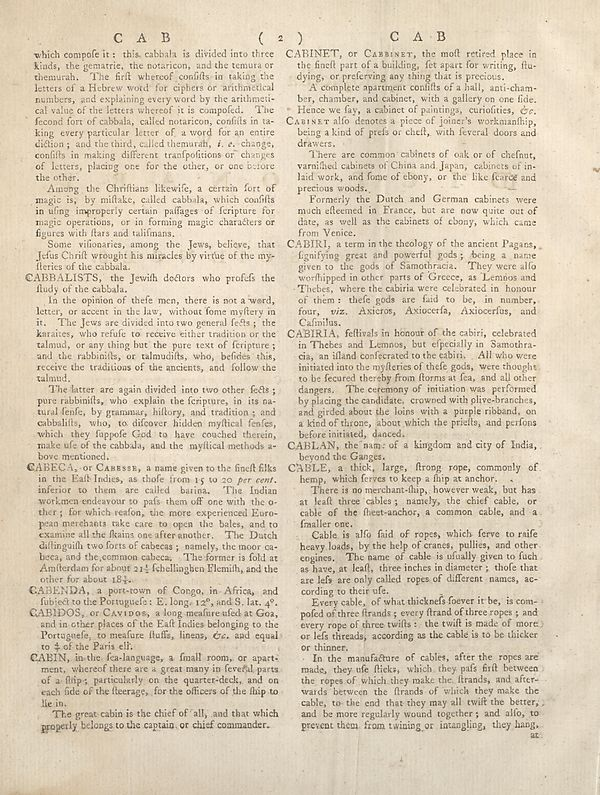
\includegraphics[width=0.85\textwidth]{../scans/page-2464-24f450326eee.jpg}
\caption*{Source scan: \texttt{page-2464-24f450326eee.jpg}}
\end{figure}
\begin{figure}[h]
\centering
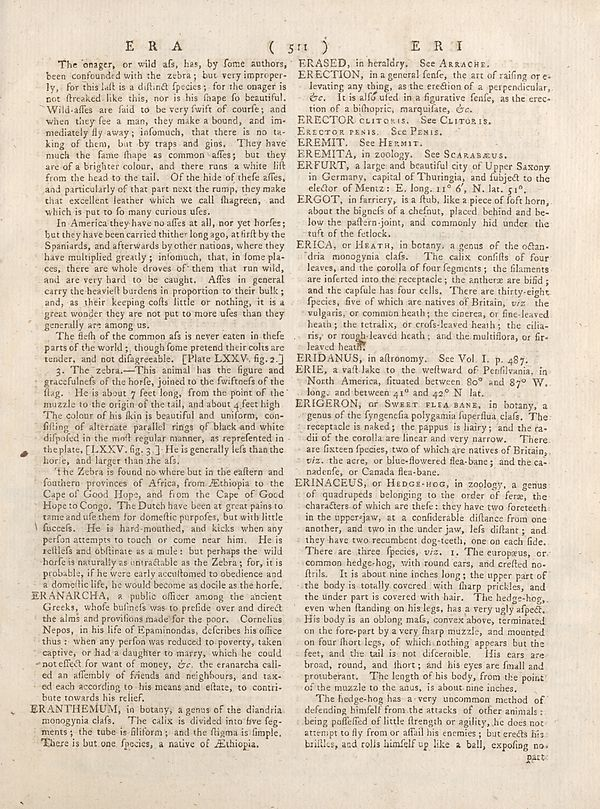
\includegraphics[width=0.85\textwidth]{../scans/page-2473-b849fb7f25f2.jpg}
\caption*{Source scan: \texttt{page-2473-b849fb7f25f2.jpg}}
\end{figure}

\end{document}
